\documentclass[5p,times,authoryear]{Config/elsarticle}
\usepackage{Config/ecrc_RIAI}

\usepackage[vietnamese]{babel}
\addto\captionsspanish{%
\def\tablename{Tabla}%
}
\usepackage[utf8]{vietnam}
\newtheorem{dl}{Định lý}
\newtheorem{hq}{Hệ quả}
\newtheorem{dn}{Định nghĩa}
\newtheorem{md}{Mệnh đề}
\newtheorem{bd}{Bổ đề}
\newtheorem{vd}{Ví dụ}
\newtheorem{tc}{Tính chất}
\newtheorem{cm}{Chứng minh}
\newtheorem{luuy}{Lưu ý}
\newtheorem{note}{Ghi nhớ}
\newtheorem{bt}{Bài tập}
\newtheorem{nx}{Nhận xét}
\newtheorem{theorem}{Theorem}
\newtheorem{remark}{Remark}
\newtheorem{proposition}{Proposition}
\newtheorem{lemma}{Lemma}
\newtheorem{definition}{Definition}
\newtheorem{proof}{Proof}
\newtheorem{example}{Example}
\newtheorem{corollary}{Corollary}
\usepackage{amsmath}       
\usepackage{tikz}
\usepackage{letterspace}
\usepackage{epstopdf}          
\usepackage{flushend}    
\usepackage{color}
\volume{38}
\firstpage{1}




%\runauth{Primer autor et al.}

%\jid{RIAI}

\jnltitlelogo{}
\usepackage{amssymb}
\usepackage[figuresright]{rotating}
\usepackage{subfigure}
\usepackage{background}
\backgroundsetup{
  scale=0.8,
  angle=0,
  opacity=0.2,  % độ mờ
  contents={%
    
\includegraphics[width=\paperwidth,height=\paperheight,keepaspectratio]{Logos/logo-noback.png}
  }
}

\newcommand{\resetsections}{
  \setcounter{section}{0}
  \setcounter{subsection}{0}
  \setcounter{subsubsection}{0}
  \setcounter{paragraph}{0}
  \setcounter{equation}{0}
  \setcounter{figure}{0}
  \setcounter{table}{0}
  \setcounter{footnote}{0}
}

\newcommand{\resetarticledata}{%
  \gdef\elsauthors{}%
  \gdef\elsaddress{}%
}

\newcommand{\resetalltheorems}{
  \setcounter{dl}{0}
  \setcounter{hq}{0}
  \setcounter{dn}{0}
  \setcounter{md}{0}
  \setcounter{bd}{0}
  \setcounter{vd}{0}
  \setcounter{tc}{0}
  \setcounter{cm}{0}
  \setcounter{luuy}{0}
  \setcounter{note}{0}
  \setcounter{bt}{0}
  \setcounter{nx}{0}
  \setcounter{theorem}{0}
  \setcounter{remark}{0}
  \setcounter{proposition}{0}
  \setcounter{lemma}{0}
  \setcounter{definition}{0}
  \setcounter{proof}{0}
  \setcounter{example}{0}
  \setcounter{corollary}{0}
}


\newcommand{\engreferences}{%
  \renewcommand{\refname}{References}%
  \renewcommand{\bibname}{References}%
}

\newcommand{\vnreferences}{%
  \renewcommand{\refname}{Tài liệu tham khảo}%
  \renewcommand{\bibname}{Tài liệu tham khảo}%
}


\newcommand{\EngArticleInfo}[5]{
\begin{flushleft}
    \rule{\textwidth}{0.4pt}\\
    \vspace{0.3cm}
    \begin{minipage}{0.35\textwidth}
     \textls[200]{\large\textsc{Info}}\\
     \rule{\textwidth}{0.2pt}
     \end{minipage}
      \hfill 
      \begin{minipage}{0.6\textwidth}
       \textls[200]{\large\textsc{Abstract}}\\
       \rule{\textwidth}{0.3pt}
        \end{minipage}
    
    \vspace{0.2cm}
    \begin{minipage}{0.35\textwidth}
        \textit{Article history:}\\
        Received: #1\\
        Accepted: #2\\
        Edited by: #3\\
        \rule{\textwidth}{0.2pt}\\
    
        \textit{Keywords:}\\
        #4
    \end{minipage} 
    \hfill
    \begin{minipage}{0.6\textwidth}
    #5
        \\
        \vspace{0.5cm}
        \hfill\copyright\ \the\year{} T\&T Reseach Club. All rights reserved.
    \end{minipage}
    
    \rule{\textwidth}{0.4pt}
\end{flushleft}
}

\newcommand{\VnArticleInfo}[5]{
\begin{flushleft}
    \rule{\textwidth}{0.4pt}\\
    \vspace{0.3cm}
    \begin{minipage}{0.35\textwidth}
     \textls[200]{\large\textsc{Thông tin}}\\
     \rule{\textwidth}{0.2pt}
     \end{minipage}
      \hfill 
      \begin{minipage}{0.6\textwidth}
       \textls[200]{\large\textsc{Tóm tắt}}\\
       \rule{\textwidth}{0.3pt}
        \end{minipage}
    
    \vspace{0.2cm}
    \begin{minipage}{0.35\textwidth}
        \textit{Lịch sử bài báo:}\\
       Ngày nhận: #1\\
        Ngày duyệt: #2\\
        Biên tập bởi: #3\\
        \rule{\textwidth}{0.2pt}\\
    
        \textit{Từ khóa:}\\
        #4
    \end{minipage} 
    \hfill
    \begin{minipage}{0.6\textwidth}
    #5
        \\
        \vspace{0.5cm}
        \hfill\copyright\ \the\year{} T\&T Reseach Club. All rights reserved.
    \end{minipage}
    
    \rule{\textwidth}{0.4pt}
\end{flushleft}
}

%Hướng dẫn một số lệnh:
%\resetsections: Chèn sau mỗi bài viết để reset chỉ mục
%\resetarticledata: Chèn sau mỗi bài viết để reset author
%\resetalltheorems: Chèn sau mỗi bài viết để reset theorem
%\engreferences: Sử dụng trước môi trường thebibliography trong bài báo tiếng Anh
%\vireferences: Sử trước môi trường thebibliography trong bài báo tiếng Việt
%\VnArticleInfo{1}{2}{3}{4}{5}: 1: Ngày nhận bài, 2: Ngày duyệt bài, 3: Tên biên tập viên, 4: Từ khóa, 5: Tóm tắt
%\EngArticleInfo{1}{2}{3}{4}{5}: Tương tự VnArticleInfo


\begin{document}

\resetsections
\resetarticledata
\resetalltheorems


\begin{frontmatter}

\title{Nguyễn Du và kiệt tác Truyện Kiều}

\author[First]{Tác giả 1}
\author[Second]{Tác giả 2}
\author[Third]{Tác giả 3}


\address[First]{Thông tin tác giả 1 }
\address[Second]{Thông tin tác giả 2}
\address[Third]{Thông tin tác giả 3}

\end{frontmatter}

\VnArticleInfo
  {01/01/2025} % 1: Ngày nhận
  {02/01/2025} % 2: Ngày duyệt
  {Tên biên tập viên} % 3: Người biên tập
  {Truyện Kiều, Nguyễn Du} %4: Từ khóa
  {Có thuyết nói Nguyễn Du viết Truyện Kiều sau khi đi sứ Trung Quốc
(1814–1820). Lại có thuyết nói ông viết trước khi đi sứ, có thể vào khoảng cuối
thời Lê đầu thời Tây Sơn.[1] Thuyết sau được nhiều người chấp nhận hơn.[2]
Ngay sau khi ra đời, Truyện Kiều được nhiều nơi khắc in và lưu hành rộng rãi.
Hai bản in xưa nhất hiện còn là bản của Liễu Văn Đường (1871) và bản của
Duy Minh Thị (1872), đều ở thời vua Tự Đức.[2] Truyện dựa theo cốt truyện
văn xuôi Kim Vân Kiều của Thanh Tâm Tài Nhân[3], lấy bối cảnh Trung Quốc
thời vua Gia Tĩnh Đế đời nhà Minh (từ năm 1521 tới năm 1567).} %5. Tóm tắt
\section{Các Môi Trường Chính}


\begin{dn}
    Nội dung Định nghĩa 
\end{dn}

\begin{dl}
   Nội dung Định lý
\end{dl}

\begin{cm}
    
\end{cm}

\begin{hq}
    Nội dung Hệ quả
\end{hq}

\begin{bd}
    Nội dung Bổ đề
\end{bd}

\begin{md}
    Nội dung Mệnh đề
\end{md}

\begin{vd}
    Nội dung Ví dụ
\end{vd}

\section{Công Thức Toán học}

Gõ công thức toán trong LaTeX có thể thực hiện bằng cú pháp inline $a^2 + b^2 = c^2$ hoặc dạng block:
\begin{equation}
    E = mc^2
\end{equation}
Ngoài ra, có thể sử dụng môi trường \texttt{align} để căn chỉnh nhiều dòng phương trình:
\begin{align}
    x + y &= 10 \\
    x - y &= 4
\end{align}
Sử dụng môi trường \texttt{align*} nếu không cần đánh số cho phương trình
\begin{align*}
    x + y &= 10 \\
    x - y &= 4
\end{align*}

\section{Chèn Hình Ảnh}

\begin{figure}[h!]
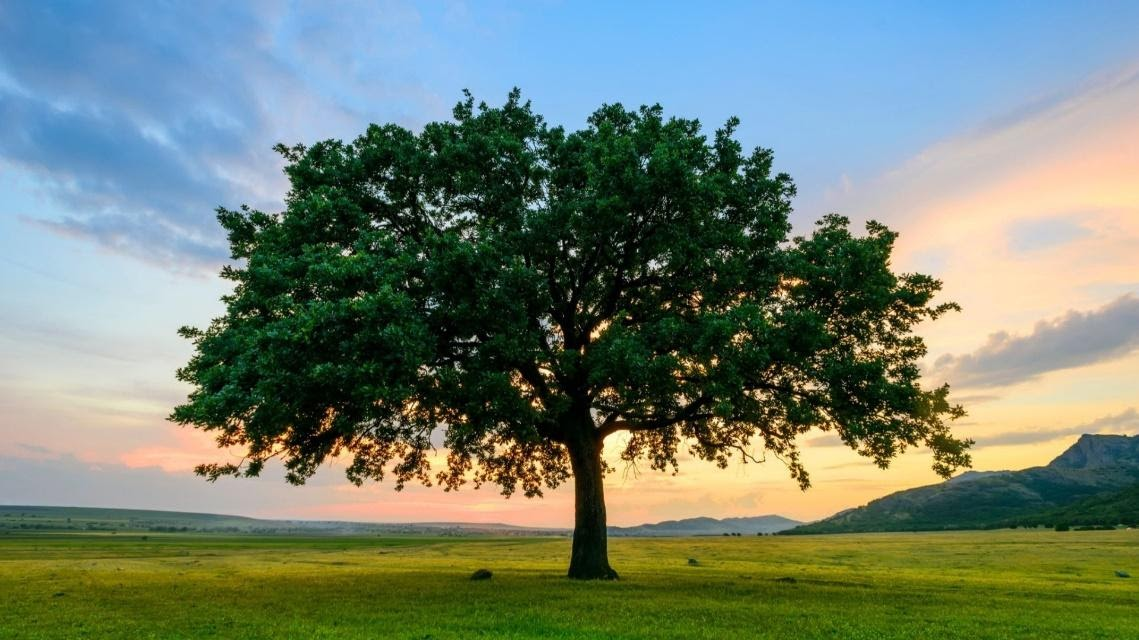
\includegraphics[width=0.7\textwidth]{Images/tree.jpg}
    \centering
    \caption{Tiêu đề ảnh}
    \label{Hình 1}
\end{figure}

\newpage
\bibliography{reference}
\bibliographystyle{plain}
\nocite{*}

\end{document}
